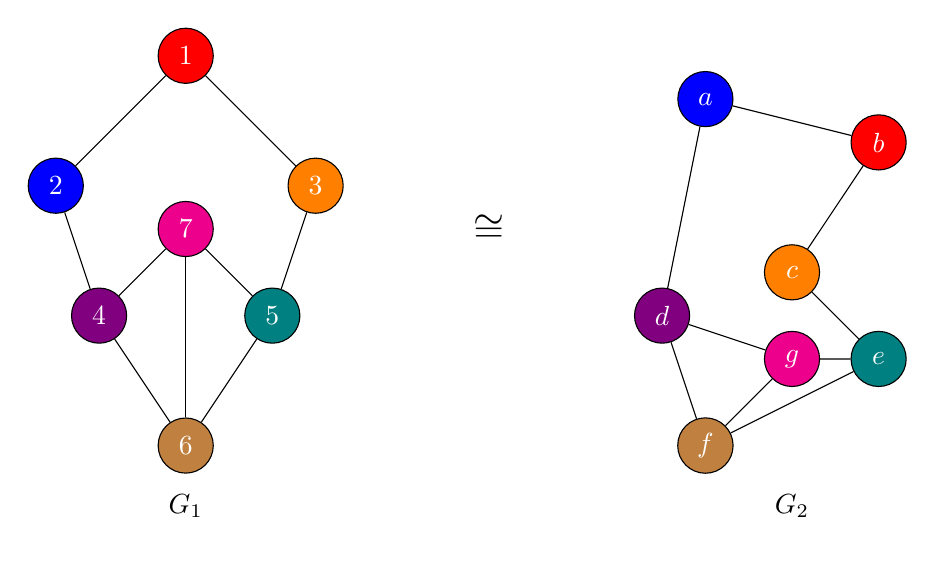
\begin{tikzpicture}[
    scale=1.1,
    every node/.style={circle, draw, minimum size=7mm}
]

\tikzset{iso/.style={fill=#1, draw=black, text=white}}

% ================= G1 =================

\node[iso=red]     (v1) at (0,2.5)   {$1$};
\node[iso=blue]    (v2) at (-1.5,1)  {$2$};
\node[iso=orange]  (v3) at (1.5,1)   {$3$};
\node[iso=violet]  (v4) at (-1,-0.5) {$4$};
\node[iso=teal]    (v5) at (1,-0.5)  {$5$};
\node[iso=brown]   (v6) at (0,-2)    {$6$};
\node[iso=magenta] (v7) at (0,0.5)   {$7$};

\draw (v1)--(v2);
\draw (v1)--(v3);
\draw (v2)--(v4);
\draw (v3)--(v5);
\draw (v4)--(v6);
\draw (v5)--(v6);
\draw (v4)--(v7);
\draw (v5)--(v7);
\draw (v6)--(v7);

\node[draw=none, rectangle] at (0,-2.7) {$G_1$};


% ================= G2 =================
% même couleur = même sommet sous f

\node[iso=blue]    (u1) at (6,2)      {$a$};
\node[iso=red]     (u2) at (8,1.5)    {$b$};
\node[iso=orange]  (u3) at (7,0)      {$c$};
\node[iso=violet]  (u4) at (5.5,-0.5) {$d$};
\node[iso=teal]    (u5) at (8,-1)     {$e$};
\node[iso=brown]   (u6) at (6,-2)     {$f$};
\node[iso=magenta] (u7) at (7,-1)     {$g$};

\draw (u1)--(u2);
\draw (u1)--(u4);
\draw (u2)--(u3);
\draw (u3)--(u5);
\draw (u4)--(u6);
\draw (u5)--(u6);
\draw (u4)--(u7);
\draw (u5)--(u7);
\draw (u6)--(u7);

\node[draw=none, rectangle] at (7,-2.7) {$G_2$};


% ================= Symbole d'isomorphisme =================

\node[draw=none, rectangle] at (3.5,0.5) {\Large $\cong$};

\end{tikzpicture}